\documentclass{article}
\usepackage{jcapstone}
\begin{document}

\title{The Skew-Normal Approximation of the Binomial Distribution}
\author{Joyce Tipping}
\date{2010}
\maketitle

\section{Introduction}

One of the most basic distributions in statistics is the binomial, $X \sim
Bin(n,p)$, with pdf

\begin{equation*}
  f_X(x) = \binom{n}{x} p^x q^{n-x}
\end{equation*}

Calculating the binomial cdf, $F_X(x) = P(X \leq x) = \sum_{k=1}^x f_X(k)$, by
hand is manageable for small $n$ but quickly becomes cumbersome as $n$ grows
even mediumly large. A common strategy is to use the normal distribution as an
approximation:

\begin{equation}
  F_X(x) \approx \Phi \left( \frac{x + 0.5 - \mu}{\sigma} \right)
\end{equation}

where $\Phi$ is the standard normal cdf and $\mu = np$ and $\sigma =
\sqrt{np(1-p)}$.

This approximation works well when either $n$ is very large (invoking the
Central Limit Theorem) or when $p$ is close to 0.5 (making $X$ roughly
symmetric). However, when $n$ is not large and $p$ is close to 0 or 1, the
binomial distribution is skewed and the normal approximation can be inaccurate;
sometimes, as demonstrated by \citet{mabs}, rather substantially. In these
cases, the skew-normal approximation can provide an alternate -- and
considerably more accurate -- method of approximation.

%\begin{equation*}
%  np(1-p) > 9
%\end{equation*}
%
%or
%
%\begin{align*}
%      np &> 5 \quad \textnormal{for} \quad  0 < p \leq 0.5, \\
%  n(1-p) &> 5 \quad \textnormal{for} \quad  0.5 < p < 1
%\end{align*}

%However, when $n$ is not large and $p$ is close to 0 or 1, the binomial
%distribution is skewed and even if the above requirements are met, the
%approximation can be inaccurate; sometimes, as demonstrated by \citet{mabs},
%rather substantially. In these cases, the skew-normal approximation can
%provide an alternate -- and considerably more accurate -- method of
%approximation.

\section{The Skew-Normal}

The skew-normal distribution is similar to the normal but with an added
parameter for skew, allowing it to lean asymmetrically to the left or right. In
this section, we'll acquaint ourselves with some of its basic properties.

\subsection{Basics}

Let $Y$ be a skew-normal distribution, with location parameter $\mu \in \R$,
scale parameter $\sigma > 0$, and shape parameter $\lambda \in \R$; we will
denote it $SN(\mu, \sigma, \lambda)$. Then $Y$ has pdf

\begin{equation} \label{eq:sn-pdf}
  f_Y(x) = \frac2\sigma \cdot \phi \left( \frac{x-\mu}{\sigma} \right) \cdot \Phi \left( \frac{\lambda(x-\mu)}{\sigma} \right)
\end{equation}

where $\phi$ is the standard normal pdf and $\Phi$ is the standard normal cdf.
Some other basic properties of $Y$, given by \citet{pewsey}, are

\begin{align}
  E(Y) &= \mu + b \delta \sigma \nonumber \\
  E(Y^2) &= \mu^2 + 2b \delta \mu \sigma + \sigma^2 \label{eq:sn-basic-properties} \\
  E(Y^3) &= \mu^3 + 3 b \delta \mu^2 \sigma + 3 \mu \sigma^2 + 3 b \delta \sigma^3 - b \delta^3 \sigma^3 \nonumber \\
  Var(Y) &= \sigma^2 (1 - b^2 \delta^2) \nonumber
\end{align}

where $b = \sqrt{\frac{2}{\pi}}$ and $\delta = \frac{\lambda}{\sqrt{1 +
\lambda^2}}$.

The $SN(0,1,\lambda)$ distribution is called the standard skew-normal; its pdf
is

\begin{equation} \label{eq:standard-sn-pdf}
  f_z(x) = 2 \cdot \phi(x) \cdot \Phi (\lambda x)
\end{equation}

Similar to the normal and standard normal, $X = \frac{Y - \mu}{\sigma}$ and $Y
= \sigma X + \mu$.

A natural question to ask is how the skew-normal relates to the normal.
Fortunately, the connection is very intuitive: When $\lambda = 0$, Equation
\eqref{eq:sn-pdf} reverts to the normal pdf:

\begin{align*}
  f_Y(x|\lambda=0) &= \frac2\sigma \cdot \phi \left( \frac{x-\mu}{\sigma} \right) \cdot \Phi(0) \\
  &= \frac2\sigma \cdot \phi \left( \frac{x-\mu}{\sigma} \right) \cdot 0.5 \\
  &= \frac1\sigma \cdot \phi \left( \frac{x-\mu}{\sigma} \right) \\
  &= \frac1\sigma \cdot \frac{1}{\sqrt{2\pi}} \;\cdot\; \exp \left( -\frac{(x-\mu)^2}{2\sigma^2} \right) \\
  &= \frac{1}{\sqrt{2\pi\sigma^2}} \;\cdot\; \exp \left( -\frac{(x-\mu)^2}{2\sigma^2} \right)
\end{align*}

\subsection{Four Properties}
\label{subsec:four-properties}

The following four properties of the skew-normal, given by \citet{main}, help
shed some light on our enigmatic new distribution:

\begin{property} \label{prop:1}
  If $Z \sim SN(0, 1, \lambda)$, then $(-Z) \sim SN(0, 1, -\lambda)$.
\end{property}

\begin{proof}
  The standard normal pdf is an even function: $\phi(-x) =
  \frac{1}{\sqrt{2\pi}}\;e^{-(-x)^2/2} = \frac{1}{\sqrt{2\pi}}\;e^{-x^2/2} =
  \phi(x)$. But the standard normal cdf, \thinspace $\Phi(x) =
  \int_{-\infty}^\infty \phi(x)$, \thinspace is not, being 0 near $-\infty$ and
  1 near $\infty$. Thus,
  
  \begin{align*}
    f_{(-Z)}(x) &= f_Z(-x) \\
    & = 2 \cdot \phi(-x) \cdot \Phi (-\lambda x) \\
    & = 2 \cdot \phi(x) \cdot \Phi (-\lambda x)
  \end{align*}

  which is the pdf of $SN(0, 1, -\lambda)$.
\end{proof}

\begin{property} \label{prop:2}
  If $Z \sim SN(0, 1, \lambda)$, then $Z^2 \sim \chi^2_1$ (chi-square with 1 degree of freedom).
\end{property}

\begin{proof}
  To prove our result, we make use of Lemma 1 in \citet{azzalini}:

  \begin{helper-lem}
    If $f_0$ is a one-dimensional probability density function symmetric about
    0, and $G$ is a one-dimensional distribution function such that $G'$ exists
    and is a density symmetric about 0, then

    \begin{equation}
      \label{eq:azzalini-perturbation-invariance}
      f(z) = 2 \cdot f_0(z) \cdot G\{w(z)\} \quad (-\infty < z < \infty)
    \end{equation}

    is a density function for any odd function $w(\cdot)$.
  \end{helper-lem}

  This lemma provides a very useful corollary:

  \begin{helper-cor}[Perturbation Invariance]
    If $Y \sim f_0$ and $Z \sim f$, then $|Y| \overset{d}{=} |Z|$, where the
    notation $\overset{d}{=}$ denotes equality in distribution.    
  \end{helper-cor}

  Let $f_0 = \phi$ and $G = \Phi$. Then, $f_z(z) = 2 \cdot \phi(z) \cdot
  \Phi(\lambda z)$ conforms to equation
  \eqref{eq:azzalini-perturbation-invariance}, and we can conclude that $phi$
  and $Z$ are equal in distribution.

%  Notice that $\phi(x)$ is a one-dimensional probability density function
%  symmetric about 0, and $\Phi(x)$ is a one-dimensional distribution function
%  such that $\Phi'$ exists and is a density symmetric about 0. Furthermore,
%  $\lambda x$ is an odd function. Thus, $f_z(z) = 2 \cdot \phi(z) \cdot
%  \Phi(\lambda z)$ conforms to equation
%  \eqref{eq:azzalini-perturbation-invariance}. With that in mind, the corollary
%  to this lemma provides a very useful result:

  We will now show that $\phi^2 \sim \chi^2_1$:

  \begin{align*}
    M_{\phi^2}(t) &= E[e^{tx^2}] \\
    &= \int_{-\infty}^\infty \; e^{tx^2} \left[ \frac{1}{\sqrt{2\pi}} e^{-x^2/2} \right] dx \\
    &= \int_{-\infty}^\infty \; \frac{1}{\sqrt{2\pi}} \; e^{tx^2 - x^2/2} \; dx \\
    &= \int_{-\infty}^\infty \; \frac{1}{\sqrt{2\pi}} \; e^{-\frac{x^2}{2}(1 - 2t)} \; dx \\
    &= \int_{-\infty}^\infty \; \frac{1}{\sqrt{2\pi}} \; e^{-\frac{1}{2}(\sqrt{1-2t} \; x)^2} \; dx \\
    \intertext{Let $u = (\sqrt{1-2t}) \, x$; then $du = (\sqrt{1-2t}) \, dx$, \enspace $dx = \frac{du}{\sqrt{1-2t}}$, \enspace and our limits become $x \to -\infty, x \to \infty \Ra
      u \to -\infty, u \to \infty$.}
    &= \int_{-\infty}^\infty \; \frac{1}{\sqrt{2\pi}} \; e^{-u^2/2} \; \left( \frac{1}{\sqrt{1-2t}} du \right) \\
    &= \frac{1}{\sqrt{1-2t}} \; \underbrace{\left( \int_{-\infty}^\infty \; \frac{1}{\sqrt{2\pi}} \; e^{-u^2/2} \; du \right)}_{\mathclap{\textnormal{$\phi(u)$ integrated over
      $(-\infty,\infty)$ = 1}}} \label{phi-pdf} \\
    &= \frac{1}{\sqrt{1-2t}}
  \end{align*}

  which is the MGF of the $\chi^2_1$. Since $Z$ is equal in distribution to
  $\phi$, we can also conclude that $Z^2 \sim \chi^2_1$. \end{proof}

\begin{property} \label{prop:3}
  As $\lambda \to \pm \infty$, \thinspace $SN(0,1,\lambda)$ tends to the half normal distribution, $\pm |N(0,1)|$.
\end{property}

To prove our theorem, it is helpful to formally define the half normal distribution:

\begin{helper-lem} \label{lem:p2-half-normal}
  Let $X \sim N(0, \sigma^2)$. Then the distribution of $|X|$ is a half-normal
  random variable with parameter $\sigma$ and

  \begin{equation*}
    f_{|X|}(x) =
    \begin{dcases*}
      0              & when $-\infty < x \leq 0$ \\
      2 \cdot f_X(x) & when $0 < x < \infty$ 
    \end{dcases*}
  \end{equation*}
\end{helper-lem}

\begin{proof}
  Let $X \sim N(0, \sigma^2)$, defined over $A = (-\infty, \infty)$. Define 
  
  \begin{equation*}
    Y = |X| =
    \begin{dcases*}
      -x & if $x < 0$ \\
      0 & if $x = 0$ \\
      x & if $x > 0$ \\
    \end{dcases*}
  \end{equation*}

  $Y$ is not one-to-one over $A$. However, we can partition $A$ into disjoint
  subsets $A_1 = (-\infty, 0)$, $A_2 = (0, \infty)$, and $A_3 = \{0\}$ such
  that $A = A_1 \cup A_2 \cup A_3$ and $Y$ is one-to-one over each $A_i$. We
  can then transform each piece separately using Theorem 6.3.2 from
  \citet{textbook}:

  On $A_1$: $y = -x \Ra x = -y$ and $\J = \left| \frac{dx}{dy} \right| = |-1|
  = 1$, yielding

  \begin{align*}
    f_Y(y) &= f_X(x) \cdot \J \\
    &= f_X(-y) \cdot 1 \\
    &= \frac{1}{\sqrt{2\pi}\sigma} \; e^{-\frac{(-y)^2}{2\sigma^2}} \\
    &= \frac{1}{\sqrt{2\pi}\sigma} \; e^{-\frac{y^2}{2\sigma^2}} \\
    &= f_X(y)
  \end{align*}

  over the domain $A_1: -\infty < x < 0 \Ra -\infty < -y < 0 \Ra 0 < y < \infty :B_1$.

  Similarly, on $A_2$: $y = x \Ra x = y$ and $\J = \left| \frac{dx}{dy}
  \right| = |1| = 1$, yielding

  \begin{align*}
    f_Y(y) &= f_X(x) \cdot \J \\
    &= f_X(y) \cdot 1 \\
    &= f_X(y)
  \end{align*}

  over the domain $A_2: 0 < x < \infty \Ra 0 < y < \infty :B_2$.

  On $A_3$, we have $x = 0 \Ra y = 0$ and $\J = \left| \frac{dx}{dy} \right| =
  |0| = 0$, yielding $f_Y(y) = f_X(x) \cdot \J = f_X(x) \cdot 0 = 0$.

  Now, by Theorem 6.3.10 from \citet{textbook}

  \begin{align}
    f_Y(y) &= \{ f_Y(y) \textrm{ over } A_1 \} + \{ f_Y(y) \textrm{ over } A_2 \} \nonumber \\
    &= f_X(y) + f_X(y) \nonumber \\
    &= 2 \cdot f_X(y) \label{eq:p2-transform-result}
  \end{align}

  over $B = B_1 \cup B_2 = (0, \infty)$, and 0 otherwise.
\end{proof}

With Lemma \ref{lem:p2-half-normal}, we can easily show our property:

\begin{proof}[Proof of Property 3]
  Let $Z \sim SN(0,1,\lambda)$. Recall that $f_Z(x) = 2 \cdot \phi(x) \cdot
  \Phi(\lambda x)$.

  Consider $\lim_{\lambda \to \infty} f_X(x)$. When $x$ is negative, $\lambda x
  \to -\infty$ and thus $\Phi(\lambda x) \to 0$. When $x$ is positive, however,
  $\lambda x \to \infty$ and $\Phi(\lambda x) \to 1$. Thus

  \begin{equation}
    \label{eq:p2-positive-half-normal}
    \lim_{\lambda \to \infty} 2 \cdot \phi(x) \cdot \Phi(\lambda x) \eq
    \begin{dcases*}
      0 & when $x \leq 0$ \\
      2 \cdot \phi(x) & when $x > 0$
    \end{dcases*}
    \eq |N(0,1)|
  \end{equation}

  In $\lim_{\lambda \to -\infty} f_X(x)$, the signs are reversed. When $x$ is
  negative, $\lambda x \to \infty$ and $\Phi(\lambda x) \to 1$. When $x$ is
  positive, $\lambda x \to -\infty$ and $\Phi(\lambda x) \to 0$. Thus,

  \begin{equation}
    \label{eq:p2-negative-half-normal}
    \lim_{\lambda \to -\infty} 2 \cdot \phi(x) \cdot \Phi(\lambda x) \eq
    \begin{dcases*}
      2 \cdot \phi(x) & when $x < 0$ \\
      0 & when $x \geq 0$
    \end{dcases*}
    \eq -|N(0,1)|
  \end{equation}
\end{proof}


\begin{property} \label{prop:4}
  The MGF of $SN(0,1,\lambda)$ is

  \begin{equation} \label{eq:p4-sn-mgf}
    M(t|\lambda) = 2 \cdot \Phi (\delta t) \cdot e^{t^2/2}
  \end{equation}
    
  where $\delta = \frac{\lambda}{\sqrt{1 + \lambda^2}}$ and $t \in (-\infty, \infty)$.
\end{property}

\begin{proof}
  According to Equation 5 in \citet{azzalini}, the MGF of $SN(\mu, \sigma^2,
  \lambda)$ is

  \begin{equation*}
    M(t) \eq E\{e^{tY}\} \eq 2 \cdot \exp \left( \mu t + \frac{\sigma^2 t^2}{2} \right) \cdot \Phi(\delta \sigma t)
  \end{equation*}

  where $\delta = \frac{\lambda}{\sqrt{1 + \lambda^2}} \in (-1, 1)$. It follows
  that the MGF of the $SN(0, 1, \lambda)$ is

  \begin{equation*}
    2 \cdot \exp \left( 0 \cdot t + \frac{1 \cdot t^2}{2} \right) \cdot \Phi(\delta \cdot 1 \cdot t) \eq 2 \cdot e^{t^2/2} \cdot \Phi(\delta t)
  \end{equation*}
\end{proof}

\section{Developing an Approximation}

Now that we have gotten to know our new distribution a little better, we can
use it to develop an approximation for the binomial.

Let $B \sim Bin(n, p)$ and $Y \sim SN(\mu, \sigma^2, \lambda)$. We will find
estimates for $\mu$, $\sigma$, and $\lambda$ by comparing the first, second,
and third moments about the mean of $B$ and $Y$.

\subsection{The Moments of the Binomial}

We begin by examining the moments of the binomial. The first two, the mean and
variance, are simply

\begin{equation*}
  E(B) = np, \quad Var(B) = np(1-p)
\end{equation*}

Having these, we can easily find

\begin{equation*}
  E(B^2) = Var(B) + [E(B)]^2 = np(1-p) + n^2p^2 = np - np^2 + n^2p^2
\end{equation*}

which we will need for the third moment. We will also need $E(B^3)$, which we
will get via the third factorial moment:

\begin{align*}
  E[B(B-1)(B-2)] &= \sum_{x=0}^n x (x-1) (x-2) \cdot \left\{ \binom{n}{x} p^x q^{n-x} \right\} \\
  &= \sum_{x=3}^n x(x-1)(x-2) \cdot \frac{n!}{x!\;(n-x)!} \; p^x q^{n-x} \\
  &= \sum_{x=3}^n \frac{n!}{(x-3)!\;(n-x)!} \; p^x q^{n-x} \\
  &= \sum_{x=3}^n n(n-1)(n-2) p^3 \cdot \frac{(n-3)!}{(x-3)!\;(n-x)!} \; p^{x-3}q^{n-x} \\
  \intertext{Let $y=x-3$. Then $x=y+3$, and $x=3 \rightarrow y=0$ and $x=n \rightarrow y=n-3$.}
  &= n(n-1)(n-2)p^3 \cdot \sum_{y=0}^{n-3} \frac{(n-3)!}{y!\;(n-(y+3))!} \; p^y q^{n-(y+3)} \\
  &= n(n-1)(n-2)p^3 \cdot \underbrace {\sum_{y=0}^{n-3} \frac{(n-3)!}{y!\;((n-3)-y)!} \; p^y q^{(n-3)-y}}_{\mathclap{\textnormal{[pdf of $Bin(n-3,p)$ summed from 0 to $n-3$] = 1}}} \\
  &= n(n-1)(n-2)p^3 \\
  &= n^3p^3 - 3n^2p^3 + 2np^3 \\
  \intertext{Further expanding the left side and solving for $E(B^3)$,}
  E \left[ B^3 - 3B^2 + 2B \right] &= n^3p^3 - 3n^2p^3 + 2np^3 \\
  E(B^3) - 3E(B^2) + 2E(B) &= \\
  E(B^3) - 3(np - np^2 + n^2p^2) + 2np &= \\
  \Rightarrow \qquad E(B^3) &= n^3p^3 - 3n^2p^3 + 2np^3 + 3np - 3np^2 + 3n^2p^2 - 2np \\
  &= n^3p^3 - 3n^2p^3 + 2np^3 - 3np^2 + 3n^2p^2 + np
\end{align*}

With these results (and a bit of elbow grease), we can obtain the third moment
without too much trouble:

\begin{align*}
  E \left( [B - E(B)]^3 \right) &= E \left( B^3 - 3B^2 E(B) + 3B [E(B)]^2 - [E(B)]^3 \right) \\
  &= E(B^3) - 3 E(B^2) E(B) + 3 E(B) [E(B)]^2 - [E(B)]^3 \\
  &= E(B^3) - 3 E(B^2) E(B) + 2 [E(B)]^3 \\
  &= (n^3p^3 - 3n^2p^3 + 2np^3 - 3np^2 + 3n^2p^2 + np) - 3np(np - np^2 + n^2p^2) + 2n^3p^3 \\
  &= \cancel{n^3p^3} - \cancel{3n^2p^3} + 2np^3 - 3np^2 + \cancel{3n^2p^2} + np - \cancel{3n^2p^2} + \cancel{3n^2p^3} - \cancel{3n^3p^3} + \cancel{2n^3p^3} \\
  &= 2np^3 - 3np^2 + np \\
  &= np(p-1)(2p-1)
\end{align*}

Our hard-earned results, restated for convenience:

\begin{align}
  E(B) &= np \nonumber \\
  E([B - E(B)]^2) &= np(1-p) \\
  E([B - E(B)]^3) &= np(p-1)(2p-1) \nonumber
\end{align}

\subsection{The Moments of the Skew Normal}

Now we'll take a look at the moments of the skew normal. Equation
\eqref{eq:sn-basic-properties} takes care of the mean and variance; again the
third moment is a little more complicated:

\begin{align*}
  E([Y - E(Y)]^3) &= E(Y^3) - 3E(Y^2)E(Y) + 2[E(Y)]^3 \\
  &= (\mu^3 + 3 b \delta \mu^2 \sigma + 3 \mu \sigma^2 + 3 b \delta \sigma^3 - b \delta^3 \sigma^3) - 3 (\mu^2 + 2b \delta \mu \sigma + \sigma^2) (\mu + b \delta \sigma) \\
  & \quad + 2\;(\mu + b \delta \sigma)^3 \\
  &= \cancel{\mu^3} + \cancel{3 b \delta \mu^2 \sigma} + \cancel{3 \mu \sigma^2} + \cancel{3 b \delta \sigma^3} - b \delta^3 \sigma^3 - \cancel{3 \mu^3} - \cancel{9 b \delta \mu^2 \sigma} -
    \cancel{6 b^2 \delta^2 \mu \sigma^2} - \cancel{3 \mu \sigma^2} \\
  & \quad - \cancel{3 b \delta \sigma^3} + \cancel{2 \mu^3} + \cancel{6 b \delta \mu^2 \sigma} + \cancel{6 b^2 \delta^2 \mu \sigma^2} + 2 b^3 \delta^3 \sigma^3 \\
  &= 2 b^3 \delta^3 \sigma^3 - b \delta^3 \sigma^3 \\
  &= b \delta^3 \sigma^3 (2b^2 - 1)
\end{align*}

We restate our results:

\begin{alignat}{4}
  E(Y) &= \mu + b \delta \sigma \;&=&\; \mu + \sigma \cdot \sqrt{\frac{2}{\pi}} \cdot \frac{\lambda}{\sqrt{1 + \lambda^2}} \nonumber \\
  E([Y - E(Y)]^2) &= \sigma^2 (1 - b^2 \delta^2) \;&=&\; \sigma^2 \left( 1 - \frac{2}{\pi} \cdot \frac{\lambda^2}{1 + \lambda^2} \right) \\
  E([Y - E(Y)]^3) &= b \delta^3 \sigma^3 (2b^2 - 1) \;&=&\; \sigma^3 \sqrt{\frac{2}{\pi}} \left( \frac{\lambda}{\sqrt{1 + \lambda^2}} \right)^3 \left( \frac{4}{\pi} - 1 \right) \nonumber
\end{alignat}

\subsection{Solving for $\mu$, $\sigma$, $\lambda$}

Now we set the two sets of moments equal to each other and, taking $n$ and $p$
as constants, solve for $\mu$, $\sigma$ and $\lambda$.

\begin{subequations}
\begin{align}
  np &= \mu + \sigma \cdot \sqrt{\frac{2}{\pi}} \cdot \frac{\lambda}{\sqrt{1 + \lambda^2}} \label{eq:first-moment-set} \\
  np(1-p) &= \sigma^2 \left( 1 - \frac{2}{\pi} \cdot \frac{\lambda^2}{1 + \lambda^2} \right) \label{eq:second-moment-set} \\
  np(p-1)(2p-1) &= \sigma^3 \sqrt{\frac{2}{\pi}} \left( \frac{\lambda}{\sqrt{1 + \lambda^2}} \right)^3 \left( \frac{4}{\pi} - 1 \right) \label{eq:third-moment-set}
\end{align}
\end{subequations}

To get $\lambda$, we divide the cube of \eqref{eq:second-moment-set} by the
square of \eqref{eq:third-moment-set}:

\begin{align}
  \frac{\sigma^6 \left( 1 - \frac{2}{\pi} \cdot \frac{\lambda^2}{1 + \lambda^2} \right)^3}{\sigma^6 \cdot \frac{2}{\pi} \left( \frac{\lambda}{\sqrt{1 + \lambda^2}} \right)^6 \left(
    \frac{4}{\pi} - 1 \right)^2} &= \frac{n^3p^3(1-p)^3}{n^2p^2(p-1)^2(2p-1)^2} \nonumber \\
  \Rightarrow \quad \frac{\left( 1 - \frac{2}{\pi} \cdot \frac{\lambda^2}{1+\lambda^2} \right)^3}{\frac{2}{\pi} \left( \frac{\lambda^2}{1+\lambda^2} \right)^3 \left( \frac{4}{\pi} - 1
    \right)^2} &= \frac{np(1-p)}{(1-2p)^2} \label{eq:solving-for-lambda}
\end{align}

The above equation \eqref{eq:solving-for-lambda} is a rational expression in
$\lambda^2$ that can be solved with either a considerable amount of manual
labor or, more efficiently, with a computer algebra system. Once we have
$\lambda^2$, then $\lambda$ is simply either the positive or negative square
root, as determined by the sign of $(1-2p)$. This can be explained with a
little assistance from Property \ref{prop:3}: When $p \to 0$, the binomial
skews left and converges toward the positive half normal, which by
\eqref{eq:p2-positive-half-normal} corresponds to a positive $\lambda$. When $p
\to 1$, the binomial skews right and converges toward the negative half normal,
which by \eqref{eq:p2-negative-half-normal} corresponds to a negative
$\lambda$. When $p = 0.5$, the binomial is symmetric and $\lambda$ is 0,
eliminating the need for a sign. Thus:

\begin{equation}
  \label{eq:lambda-solved}
  \lambda = \textnormal{\{sign of $(1-2p)$\}} \sqrt{\lambda^2}
\end{equation}

%\textbf{\textit{Note to Dr. Guffey:} I am trying to find an algebraic reason
%for the sign, but I'm not seeing it in equation \eqref{eq:solving-for-lambda}
%nor its algebraic expansion, which I put in in appendix
%\ref{sec:solving-for-lambda} as it ended up providing little insight into this
%conclusion.}

Having secured $\lambda$, we can find $\sigma$ using
\eqref{eq:second-moment-set}:

\begin{equation}
  \label{eq:sigma-solved}
  np(1-p) = \sigma^2 \left( 1 - \frac{2}{\pi} \cdot \frac{\lambda^2}{1 + \lambda^2} \right) \quad\Rightarrow\quad
  \sigma = \sqrt{\frac{np(1-p)}{1 - \frac{2}{\pi} \cdot \frac{\lambda^2}{1 + \lambda^2}}}
\end{equation}

Similarly, with both $\lambda$ and $\sigma$, a simple rearrangement of
\eqref{eq:first-moment-set} yields $\mu$:

\begin{equation}
  \label{eq:mu-solved}
  np = \mu + \sigma \cdot \sqrt{\frac{2}{\pi}} \cdot \frac{\lambda}{\sqrt{1 + \lambda^2}} \quad\Rightarrow\quad
  \mu = np - \sigma \cdot \sqrt{\frac{2}{\pi}} \cdot \frac{\lambda}{\sqrt{1 + \lambda^2}}
\end{equation}

When $p = 0.5$, we would expect the binomial to be perfectly symmetrical and
the mean therefore to be $n/2$. From \eqref{eq:mu-solved}, this implies that
$\sigma \cdot \sqrt{\frac{2}{\pi}} \cdot \frac{\lambda}{\sqrt{1 + \lambda^2}} =
0 \Ra$ either $\sigma = 0$ or $\lambda = 0$. Since the former is impossible, we
must conclude the latter, which brings us back to the normal distribution.

%\textbf{\textit{Another note to Dr. Guffey:} The author mentions here that when
%$p=0.5$, it forces $\lambda$ to be 0, bringing us back to the regular normal
%approximation. This seems like it ought to be a simple fact, but I can't figure
%out how he's getting it from these equations. He refers to his equation (c),
%which is my equation \eqref{eq:mu-solved}. Substituting $p=0.5$ into
%\eqref{eq:mu-solved}, however, doesn't get me anywhere; neither does
%substituting $p=0.5$ into \eqref{eq:sigma-solved} and then substituting that
%into \eqref{eq:mu-solved}. And as far as I can tell, equation
%\eqref{eq:lambda-solved} is for all practical purposes useless. Alas.}

\subsection{Restrictions}

To obtain an estimate for $\lambda$, we must put a few restrictions on $n$ and
$p$.

If we let $u = \frac{\lambda^2}{1+\lambda^2}$ and $v = 1/u$, we can rewrite the
left hand side of \eqref{eq:solving-for-lambda} as

\begin{gather}
  \left. \left( 1 - \frac{2}{\pi} u \right)^3 \middle/ \frac{2}{\pi} u^3 \left( \frac{4}{\pi} - 1 \right)^2 \right. \nonumber \\
  \left( 1 - \frac{2}{\pi} u \right)^3 \cdot v^3 \cdot \frac{\pi}{2} \cdot \left( \frac{\pi}{4-\pi} \right)^2 \nonumber \\
  \left[ v \left( 1 - \frac{2}{\pi} u \right) \right]^3 \left( \frac{\pi^3}{2(4-\pi)^2} \right) \nonumber \\
  \left( v - \frac{2}{\pi} \right)^3 \left( \frac{\pi^3}{2(4-\pi)^2} \right) \label{eq:lhs-solving-for-lambda}
\end{gather}

we can see that it is increasing in $v$, which is always $\geq 1$. Therefore:

\begin{equation}
  \min_{v} \textnormal{\{Eq. \ref{eq:lhs-solving-for-lambda}\}} = \textnormal{\{Eq. \ref{eq:lhs-solving-for-lambda}\}} |_{v=1} = 
  \left( 1 - \frac{2}{\pi} \right)^3 \left( \frac{\pi^3}{2(4-\pi)^2} \right) = 1.009524 \approx 1
\end{equation}

This means that the right hand side of \eqref{eq:solving-for-lambda}, which is
supposed to be equal to the left hand side of \eqref{eq:solving-for-lambda},
can't ever be less than 1. Unfortunately, it sometimes is; in particular,
$\frac{np(1-p)}{(1-2p)^2} \to 0$ both when $p \to 0$ and $p \to 1$. So if we
want a solution, we must restrict $n$ and $p$ such that

\begin{align}
  \textnormal{\{right hand side of \eqref{eq:solving-for-lambda}\}} &\geq \textnormal{\{min of left hand side of \eqref{eq:solving-for-lambda}\}} \nonumber \\
  \frac{np(1-p)}{(1-2p)^2} &\geq 1 \nonumber \\
  np(1-p) &\geq (1-2p)^2 \label{eq:solving-the-restriction}
\end{align}

From here, given a constant $p$, finding $n$ is very simple:

\begin{equation}
  n \geq \frac{(1-2p)^2}{p(1-p)} \label{eq: n for a given p}
\end{equation}

Figure \ref{fig:sn-restriction-least-n} shows the least sample size required to
estimate $\lambda$, given a fixed $p$. As expected, the least $n$ is quite
large when $p$ is small and $\to 0$ as $p \to 0.5$. For example, when $p =
0.01$, $n \geq 98$; but at $p = 0.2$, $n$ must only be $\geq 3$, a trivial
requirement to meet.

\begin{figure}
  \centering
  \subfloat[Least possible $n$, given a fixed $p$]{\label{fig:sn-restriction-least-n}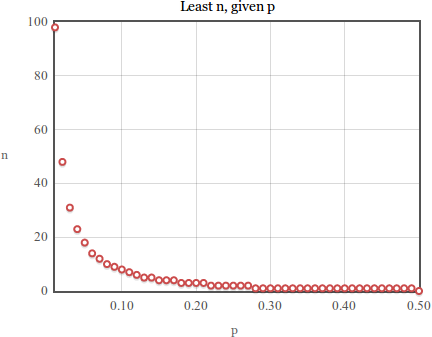
\includegraphics[width=0.45\textwidth]{../graphs/images/restriction-least-n.png}}
  \quad
  \subfloat[Range of possible $p$, given a fixed $n$]{\label{fig:sn-restriction-p-range}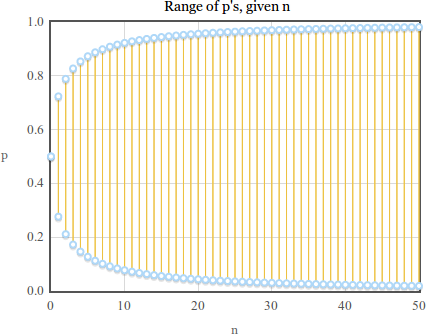
\includegraphics[width=0.45\textwidth]{../graphs/images/restriction-p-range.png}}
  \caption{Restrictions on $n$ and $p$ for estimating $\lambda$}
  \label{fig:sn-restriction}
\end{figure}

It is also possible to fix $n$ and solve for $p$. We return to
\eqref{eq:solving-the-restriction} for further factoring

\begin{align}
  np - np^2 &\geq 1 - 4p + 4p^2 \nonumber \\
  1 - 4p + 4p^2 - np + np^2 &\leq 0 \nonumber \\
  (n+4)p^2 - (n+4)p + 1 &\leq 0 \label{eq: solving for p}
\end{align}

and apply the quadratic formula with $a = n+4$, $b = -(n+4)$, and $c = 1$:

\begin{gather*}
  \frac{(n+4) \pm \sqrt{(n+4)^2 - 4 \cdot (n+4) \cdot 1}}{2(n+4)} \\
  \frac{(n+4) \pm \sqrt{n^2 + 8n + 16 - 4n - 16}}{2(n+4)} \\
  \frac{(n+4) \pm \sqrt{n^2 + 4n}}{2(n-4)} \\
  \frac{n+4}{2(n+4)} \pm \frac12 \sqrt{\frac{n(n+4)}{(n+4)^2}} \\
  \frac12 \pm \frac12 \sqrt{\frac{n}{n+4}}
\end{gather*}

Let $r_1 = \frac12 - \frac12 \sqrt{\frac{n}{n+4}}$ and $r_2 = \frac12 + \frac12
\sqrt{\frac{n}{n+4}}$. (Note that $r_1 < r_2$.) Now we can rewrite \eqref{eq:
solving for p} as

\begin{equation*}
  (p - r_1)(p - r_2) \leq 0
\end{equation*}

Examining the left hand side, when $p < r_1$, both terms are negative and so
their product is positive; when $p > r_2$, both terms are positive, again
leading the product to be positive. Therefore, our solution lies where $r_1
\leq p \leq r_2$, or more explicitly:

\begin{equation}
 \frac12 - \frac12 \sqrt{\frac{n}{n+4}} \; \leq \; p \; \leq \; \frac12 + \frac12 \sqrt{\frac{n}{n+4}}
\end{equation}

As shown in figure \ref{fig:sn-restriction-p-range}, this interval grows
quickly as $n$ increases, and for sufficiently large $n$, it becomes almost
$(0, 1)$. For example, when $n=100$, our interval is $(0.00971, 0.99029)$; when
$n=500$, it is (0.00199, 0.99801).

For $p$ so close to 0 or 1 that this solution will not work, our authors
suggest a Poission approximation.

\section{Demonstrating Improved Accuracy}

Having taken the trouble to develop our skew-normal approximation for the
binomial, we now justify our efforts by demonstrating its improved accuracy
over the regular normal approximation.

\subsection{Visual Comparison}

The first, and most obvious, way of judging accuracy is by visual inspection.
Figures \ref{fig:comparison-n25}, \ref{fig:comparison-n50}, and
\ref{fig:comparison-n100} compare the binomial, normal, and skew-normal at
small values of $p$ for $n=25$, $n=50$, and $n=100$, respectively. It is not
hard to see that, especially at very small $n$ and $p$, our skew-normal curve
follows the shape of the binomial much more accurately.

\begin{figure}
  \centering
  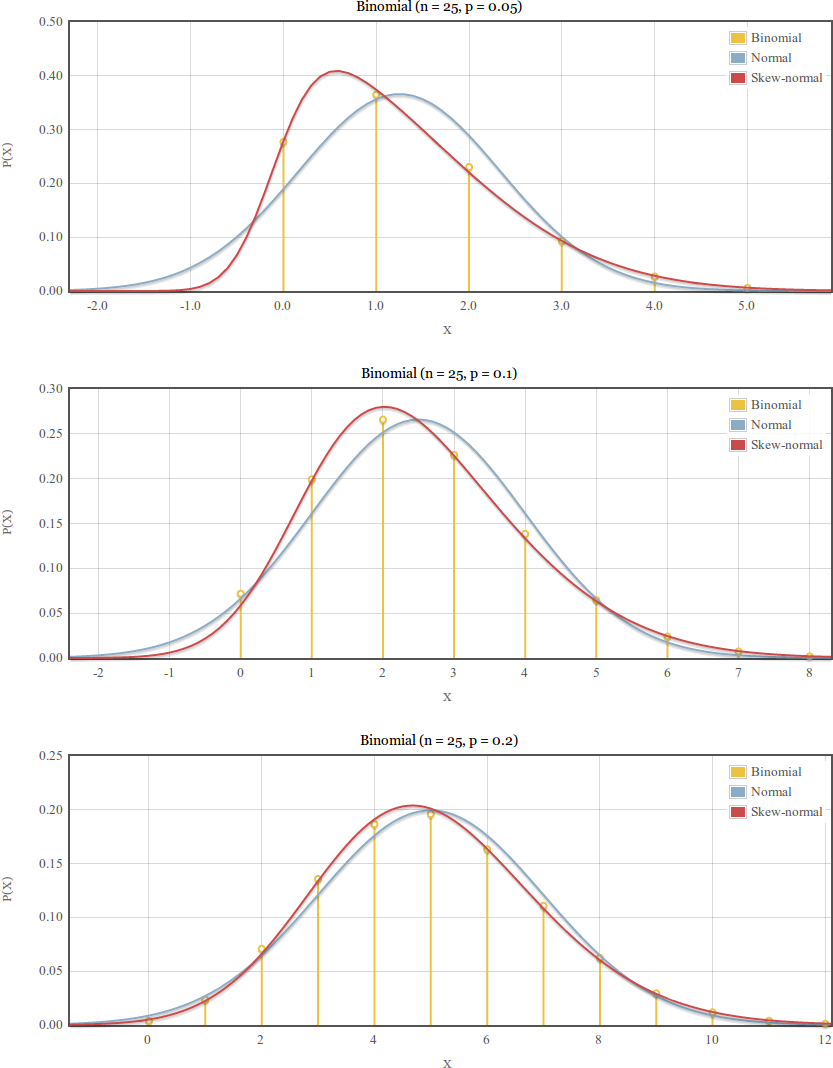
\includegraphics[width=\textwidth]{../graphs/images/comparison-n25.png}
  \caption{Binomial, normal, and skew-normal, $n=25$}
  \label{fig:comparison-n25}
\end{figure}

\begin{figure}
  \centering
  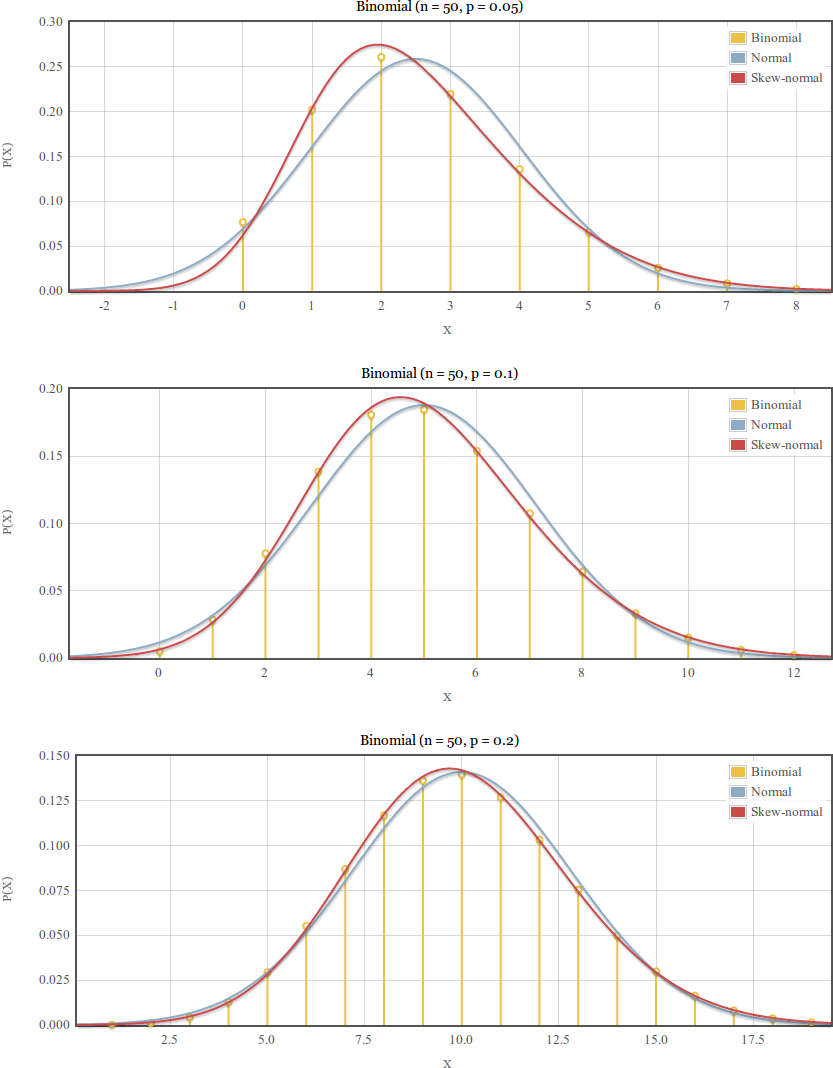
\includegraphics[width=\textwidth]{../graphs/images/comparison-n50.png}
  \caption{Binomial, normal, and skew-normal, $n=50$}
  \label{fig:comparison-n50}
\end{figure}

\begin{figure}
  \centering
  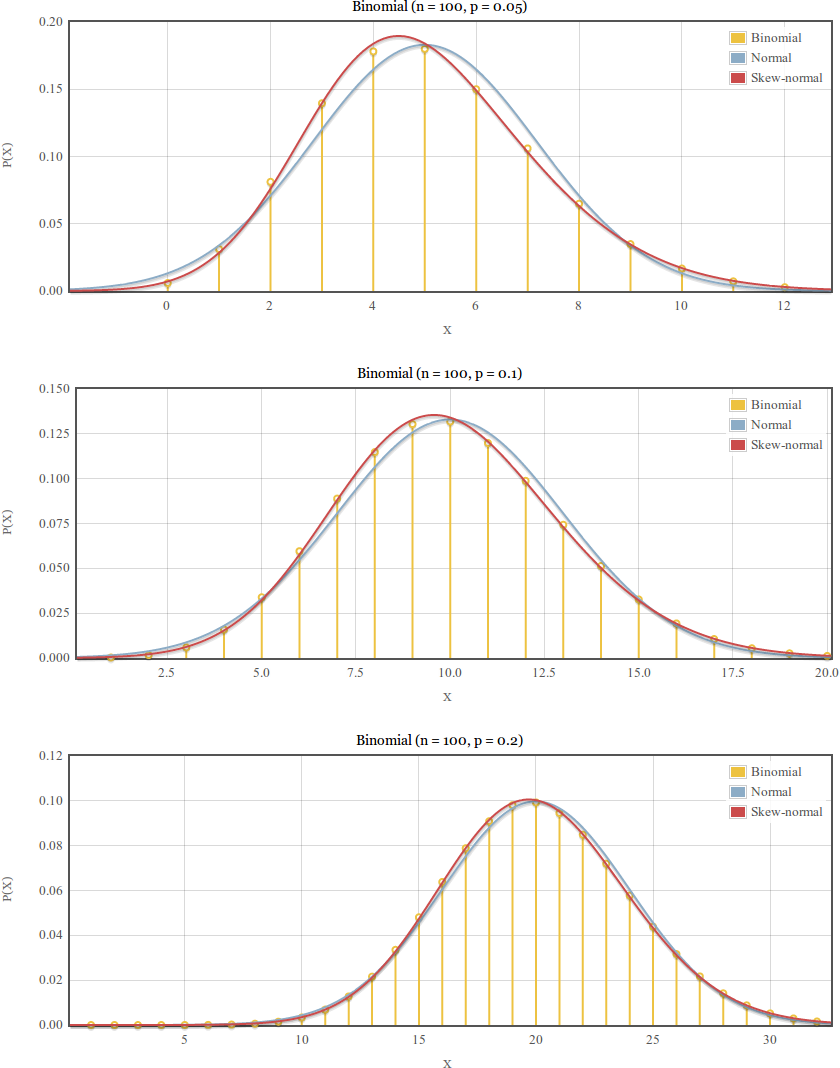
\includegraphics[width=\textwidth]{../graphs/images/comparison-n100.png}
  \caption{Binomial, normal, and skew-normal, $n=100$}
  \label{fig:comparison-n100}
\end{figure}

\subsection{Maximal Absolute Error}

Another more numerical method would be to compare the maximal absolute errors
of our two approximations, defined by \citet{mabs} as

\begin{equation}
  \textnormal{MABS}(n, p) \eq \max_{k \in \{0, 1,...,n\}} \left| F_{B(n,p)} (k) -  F_{\textnormal{appr}(n,p)}(k + 0.5) \right|
\end{equation}

where $F_{B(n,p)}$ is the cdf of the binomial and $F_{\textnormal{appr}(n,p)}$
is the cdf of either the normal or skew-normal approximation; the 0.5 is a
continuity correction.

\begin{figure}
  \centering
  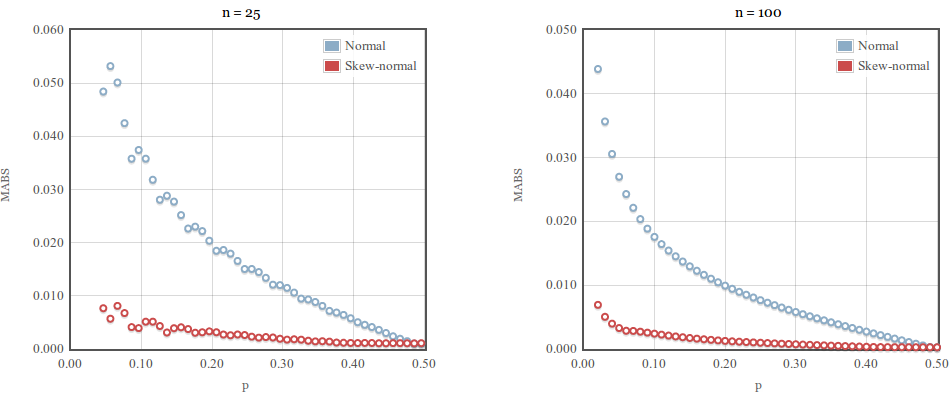
\includegraphics[width=\textwidth]{../graphs/images/mabs-fixed-n.png}
  \caption{MABS as a function of p}
  \label{fig:mabs-fixed-n}
\end{figure}

\begin{figure}
  \centering
  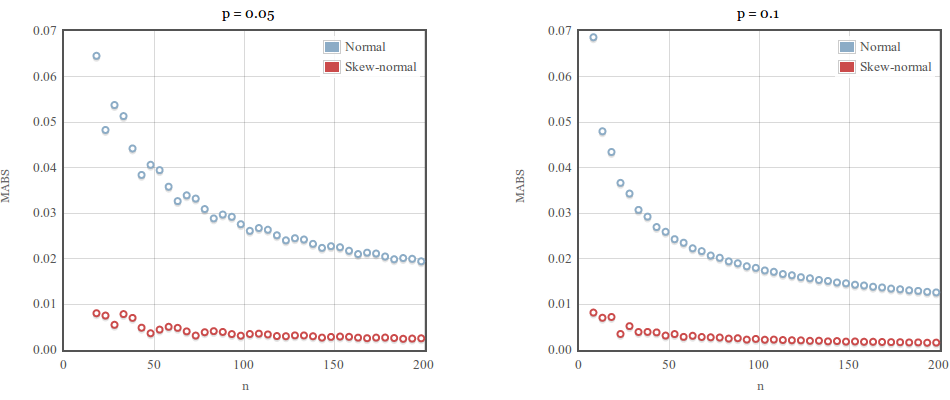
\includegraphics[width=\textwidth]{../graphs/images/mabs-fixed-p.png}
  \caption{MABS as a function of n}
  \label{fig:mabs-fixed-p}
\end{figure}

Figure \ref{fig:mabs-fixed-n} shows the MABS as a function of $p$, for $n=25$
and $n=100$. Figure \ref{fig:mabs-fixed-p}, on the other hand, shows the MABS
as a function of $n$, for $p=0.05$ and $p=0.1$. Again, the skew-normal
outperforms the normal considerably in the extreme ranges, with the two
approximations converging as $n \rightarrow \infty$ or $p \rightarrow 0.5$.

\clearpage


\bibliography{/home/joycetipping/projects/capstone/pieces/bibliography/bibliography.bib}
\bibliographystyle{plainnat}
\end{document}
